% HiLRP method overview (CVPR-style): (a) one conservation-valid backward pass
% over a hierarchical/hybrid ViT, (b) CP-LRP attention block zoom, (c) patch
% merging rule zoom, (d) the four-primitive legend. Colors match
% attnlrp_propagation.tex (P1 linear blue, P2 bilinear orange, P3 gate purple,
% P4 reindex green, relevance red).
% Compile: pdflatex hilrp_pipeline.tex   (from figures/hilrp/, needs hilrp_fig_*.png)
\documentclass[tikz,border=10pt]{standalone}
\usepackage[T1]{fontenc}
\usepackage{helvet}
\usepackage{amsmath}
\usepackage{graphicx}
\renewcommand{\familydefault}{\sfdefault}
\usetikzlibrary{positioning,arrows.meta,calc,backgrounds,fit}

\definecolor{linC}{RGB}{31,78,145}
\definecolor{bilC}{RGB}{192,96,10}
\definecolor{gateC}{RGB}{122,44,140}
\definecolor{permC}{RGB}{34,110,50}
\definecolor{relC}{RGB}{176,20,30}

\begin{document}
\begin{tikzpicture}[
  op/.style={draw, rounded corners=2pt, minimum height=9mm, minimum width=17mm,
             align=center, font=\small, line width=0.9pt, fill=white},
  lin/.style={op, draw=linC, fill=linC!8},
  bil/.style={op, draw=bilC, fill=bilC!12},
  gate/.style={op, draw=gateC, fill=gateC!8},
  perm/.style={op, draw=permC, fill=permC!8},
  io/.style={op, draw=black!60, fill=black!4},
  stage/.style={op, draw=black!65, fill=black!6, minimum height=11mm},
  fwd/.style={-{Stealth[length=2.2mm]}, line width=0.8pt, draw=black!75},
  rel/.style={-{Stealth[length=2.6mm]}, line width=1.2pt, draw=relC},
  flab/.style={font=\scriptsize, fill=white, inner sep=1pt},
  rlab/.style={font=\scriptsize, text=relC, fill=white, inner sep=1pt},
  rul/.style={font=\scriptsize, align=center},
  grid/.style={font=\scriptsize, text=black!55},
  ptitle/.style={font=\small\bfseries, anchor=north west},
  panel/.style={draw=black!35, rounded corners=4pt, line width=0.7pt, fill=black!2},
]

% =================== (a) main pipeline ===================
\node[ptitle] at (-1.3, 11.9)
  {(a) HiLRP: one conservation-valid backward pass over any hierarchical or hybrid ViT};

\node[inner sep=0, draw=black!60, line width=0.8pt] (img) at (0.0, 9.6)
  {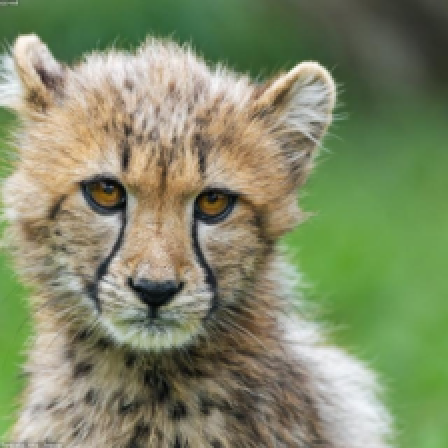
\includegraphics[width=2.0cm]{hilrp_fig_input.png}};
\node[font=\scriptsize, above=1pt of img] {input $x$};

\node[lin]   (pe) at (3.4, 9.6)  {Patch Embed\\[-2pt]\scriptsize conv};
\node[stage] (s1) at (6.4, 9.6)  {Stage 1\\[-2pt]\scriptsize $\times L_1$ blocks (b) $\cdot$ $56^2$};
\node[perm]  (pm) at (9.5, 9.6)  {Patch\\[-2pt]Merging (c)};
\node[stage] (s2) at (12.4, 9.6) {Stage 2\\[-2pt]\scriptsize $28^2$};
\node[font=\normalsize] (dots) at (14.4, 9.6) {$\cdots$};
\node[stage] (s4) at (16.3, 9.6) {Stage 4\\[-2pt]\scriptsize $7^2$};
\node[op]    (hd) at (19.3, 9.6) {LN $\cdot$ pool\\[-2pt]$\cdot$ head};
\node[io, minimum width=13mm] (lg) at (21.9, 9.6) {$f_c(x)$};

\node[grid] at (14.4, 10.1) {\tiny (merge between stages)};

\node[rul, text=linC]  at (3.4, 10.55)  {P1: $\gamma$ rule};
\node[rul, text=black!60] at (6.4, 10.75) {CP attention, identity LN,\\$\gamma$ MLP, residual exact};
\node[rul, text=permC] at (9.5, 10.55)  {P4 concat + P1 $z^+$};
\node[rul, text=black!60] at (19.3, 10.55) {P3 identity, P1};

\draw[fwd] (img) -- (pe);
\draw[fwd] (pe) -- (s1);
\draw[fwd] (s1) -- (pm);
\draw[fwd] (pm) -- (s2);
\draw[fwd] (s2) -- (dots);
\draw[fwd] (dots) -- (s4);
\draw[fwd] (s4) -- (hd);
\draw[fwd] (hd) -- (lg);

% backward relevance
\draw[rel] (lg.south) to[bend left=25] node[rlab, below=2pt]{seed $R := f_c(x)$} (hd.south);
\draw[rel] (hd.south) to[bend left=25] (s4.south);
\draw[rel] (s4.south) to[bend left=18] (s2.south);
\draw[rel] (s2.south) to[bend left=25] node[rlab, below=2pt]{$z^+$ split, regroup exact} (pm.south);
\draw[rel] (pm.south) to[bend left=25] (s1.south);
\draw[rel] (s1.south) to[bend left=25] node[rlab, below=2pt]{value path (b)} (pe.south);

% pixel output: real HiLRP map
\node[inner sep=0, draw=relC, line width=0.9pt] (heat) at (0.0, 6.6)
  {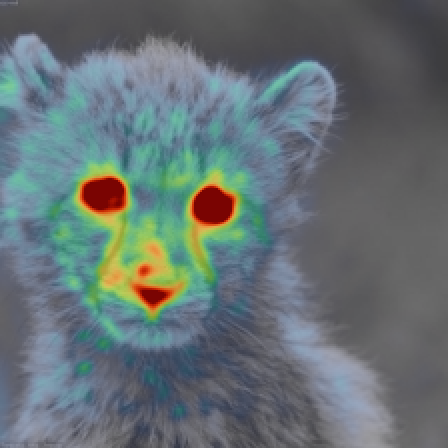
\includegraphics[width=2.0cm]{hilrp_fig_heatmap.png}};
\node[font=\scriptsize, text=relC, anchor=west, align=left] at (1.2, 6.7)
  {attribution $R(x)$\\[-1pt]{\tiny real HiLRP map (PVT-v2-b2)}\\[-1pt]
   {\tiny pixel step: $\gamma$ denoising,}\\[-2pt]{\tiny deviation $0.82\pm0.08$}};
\draw[rel] (pe.south west) to[out=-140, in=20]
  node[rlab, pos=0.5, above left=0pt]{$\gamma$ conv $\to$ pixels} (heat.north east);

% conservation ribbon
\node[draw=relC!70, rounded corners=3pt, fill=relC!4, inner sep=4pt,
      font=\scriptsize, align=center] at (13.6, 7.1)
  {\textbf{Token-level conservation at every interface:} $\sum_j R_j = f_c(x)$.
   Float64 reference: patch merge $3{\times}10^{-16}$, shifted-window mask leak $\sim10^{-43}$,
   permutations exact (Lemma 2).};

% =================== (b) CP-LRP attention zoom ===================
\node[panel, minimum width=14.0cm, minimum height=6.0cm, anchor=south west] (pb) at (-1.3, -0.75) {};
\node[ptitle] at (-1.15, 5.0) {(b) One block: CP-LRP attention, relevance takes the value path};

\node[io]   (bx)  at (0.0, 1.9)  {tokens\\$X$};
\node[lin, minimum width=11mm, fill=linC!4, draw=linC!55] (bwq) at (2.2, 3.3) {$W_Q$};
\node[lin, minimum width=11mm, fill=linC!4, draw=linC!55] (bwk) at (2.2, 2.1) {$W_K$};
\node[lin, minimum width=11mm] (bwv) at (2.2, 0.6) {$W_V$};
\node[bil, minimum width=15mm, fill=bilC!5, draw=bilC!55]  (bqk) at (4.5, 2.9) {$QK^{\top}\!/\sqrt{d}$};
\node[gate, minimum width=13mm, fill=gateC!5, draw=gateC!55] (bsm) at (6.8, 2.9) {softmax};
\node[bil]  (bav) at (8.6, 0.9)  {$A \cdot V$};
\node[lin, minimum width=11mm]  (bwo) at (10.6, 0.9) {$W_O$};
\node[io, minimum width=11mm]   (bout) at (12.2, 0.9) {$y$};

\draw[fwd] (bx) -- (bwq);
\draw[fwd] (bx) -- (bwk);
\draw[fwd] (bx) -- (bwv);
\draw[fwd] (bwq) -- (bqk);
\draw[fwd] (bwk) -- (bqk);
\draw[fwd] (bqk) -- (bsm);
\draw[fwd] (bsm.east) to[out=0, in=90] node[flab, pos=0.3, right=1pt]{$A$} (bav.north);
\draw[fwd] (bwv.east) -| node[flab, pos=0.2, above=1pt]{$V$} (bav.south west);
\draw[fwd] (bav) -- node[flab, above=1pt, text=permC]{\tiny merge: P4} (bwo);
\draw[fwd] (bwo) -- (bout);

% annotations
\node[rul, text=black!45] at (4.5, 3.9) {query/key path: receives no relevance};
\node[rul, text=linC] at (2.2, 4.35) {P1: $\gamma$ rule};
\node[rul, text=gateC, anchor=west, align=left] at (9.55, 3.55)
  {$A$ detached (P3): constant\\gate, carries no relevance};
\draw[black!40, line width=0.5pt] (9.5, 3.35) -- (8.85, 2.5);
\node[rul, text=bilC, anchor=west, align=left] at (9.55, 2.2)
  {P2, gate detached:\\linear in $V$, conserves};

% backward: value path only
\draw[rel] (bout.south) to[bend left=30] node[rlab, below=2pt]{$R^{(y)}$} (bwo.south);
\draw[rel] (bwo.south) to[bend left=30] (bav.south east);
\draw[rel] (bav.south) to[out=-120, in=-15]
  node[rlab, pos=0.5, below=2pt]{full $R$ through the value path}
  (bwv.south east);
\draw[rel] (bwv.west) to[bend left=20] node[rlab, pos=0.55, below left=0pt]{$R^{(X)}$} (bx.south);

% =================== (c) patch merging zoom ===================
\node[panel, minimum width=7.3cm, minimum height=6.0cm, anchor=south west] (pc) at (12.9, -0.75) {};
\node[ptitle] at (13.05, 5.0) {(c) Patch merging: exact rule};

\node[draw=black!60, fill=linC!14, minimum size=5.5mm, font=\scriptsize] (t0) at (13.9, 3.45) {$x_0$};
\node[draw=black!60, fill=bilC!18, minimum size=5.5mm, font=\scriptsize] (t1) at (14.6, 3.45) {$x_1$};
\node[draw=black!60, fill=permC!14, minimum size=5.5mm, font=\scriptsize] (t2) at (13.9, 2.75) {$x_2$};
\node[draw=black!60, fill=gateC!12, minimum size=5.5mm, font=\scriptsize] (t3) at (14.6, 2.75) {$x_3$};
\node[grid] at (14.25, 2.2) {$2{\times}2$ tokens};
\node[draw=relC!60, dashed, rounded corners=1pt, inner sep=2pt,
      fit=(t0)(t1)(t2)(t3)] (tg) {};

\node[perm, minimum width=12mm, minimum height=16mm] (cc) at (16.4, 3.1) {concat\\[-2pt]\scriptsize P4};
\node[lin, minimum width=10mm] (cw) at (18.1, 3.1) {$W$\\[-2pt]\scriptsize P1 $z^+$};
\node[draw=black!70, fill=black!10, minimum size=6.5mm, font=\scriptsize] (cy) at (19.5, 3.1) {$y$};

\draw[fwd] (tg.east) -- (cc.west);
\draw[fwd] (cc) -- (cw);
\draw[fwd] (cw) -- (cy);

% backward: one arc over the top, split by z+ shares
\draw[rel] (cy.north) to[out=135, in=45, looseness=0.75]
  node[rlab, pos=0.5, below=2pt]{$R_y$ split by $z^+$ shares}
  (tg.north);

\node[rul, text=relC, anchor=west] at (13.15, 1.35)
  {$R_{x_k}=\sum_c \dfrac{x_k W^+_{k,c}}{\sum_{k'} x_{k'} W^+_{k',c}+\epsilon}\,R_{y,c}$};
\node[rul, text=black!55, anchor=west, align=left] at (13.15, 0.35)
  {\tiny conserves to $3{\times}10^{-16}$; un-concat regroup and\\[-3pt]
   \tiny cyclic shift are permutations: exact, no leak};

% =================== (d) primitive legend ===================
\node[panel, minimum width=6.7cm, minimum height=6.0cm, anchor=south west] (pd) at (20.5, -0.75) {};
\node[ptitle] at (20.65, 5.0) {(d) Four conserving primitives};

\fill[linC!25] (20.8, 4.0) rectangle ++(0.26,0.26);
\draw[linC, line width=0.8pt] (20.8, 4.0) rectangle ++(0.26,0.26);
\node[rul, anchor=west, align=left] at (21.2, 4.13)
  {\textbf{P1 linear}: Q/K/V/out, MLP, conv,\\pool $\to$ $\varepsilon/\gamma$ rule};
\fill[bilC!25] (20.8, 3.1) rectangle ++(0.26,0.26);
\draw[bilC, line width=0.8pt] (20.8, 3.1) rectangle ++(0.26,0.26);
\node[rul, anchor=west, align=left] at (21.2, 3.23)
  {\textbf{P2 bilinear}: $QK^{\top}$, $A{\cdot}V$, linear attn.\\$\to$ split, or CP: detach one factor};
\fill[gateC!25] (20.8, 2.2) rectangle ++(0.26,0.26);
\draw[gateC, line width=0.8pt] (20.8, 2.2) rectangle ++(0.26,0.26);
\node[rul, anchor=west, align=left] at (21.2, 2.33)
  {\textbf{P3 normalize/gate}: softmax, LN,\\denominators $\to$ detach $\to$ identity};
\fill[permC!25] (20.8, 1.3) rectangle ++(0.26,0.26);
\draw[permC, line width=0.8pt] (20.8, 1.3) rectangle ++(0.26,0.26);
\node[rul, anchor=west, align=left] at (21.2, 1.43)
  {\textbf{P4 reindex}: heads, windows, shifts,\\merge $\to$ permutation, exact};

\node[rul, text=black!65, anchor=west, align=left, font=\scriptsize\itshape]
  at (20.8, 0.35) {A new ViT is a new arrangement of the same\\four: covered by construction, no new derivation.};

\end{tikzpicture}
\end{document}
